\chapter{Diseño e implementación}
\label{cap:DisenioImplementacion}

En este capítulo se presenta la arquitectura de hardware y software del dispositivo de captura, como así también del generador de señal MVB desarrollado para probar el dispositivo de captura sin necesidad de conectarlo en una formación ferroviaria.

\section{Arquitectura de hardware}
\label{sec:hardware}

Como se muestra en la figura~\ref{fig:conexion}, el dispositivo de captura tiene dos conectores DE-9 compatibles con el medio EMD. De esta manera se lo puede conectar a un segmento MVB entre dos dispositivos cualesquiera.

\begin{figure}[htbp]
	\centering
    {
        \fontfamily{phv}
        \fontsize{8pt}{8pt}\selectfont
        \input{./Figures/conexion.pdf_tex}
    }
	\caption{Conexión del dispositivo de captura en un segmento EMD.}
    \label{fig:conexion}
\end{figure}

En la figura~\ref{fig:bloques} se muestra un diagrama de la arquitectura del dispositivo de captura.
Se dejan en corto circuito las líneas de transmisión (ver figura~\ref{fig:pines}), de forma tal de que el dispositivo opere en forma pasiva. Salvando la impedancia que agrega a la línea, el dispositivo de captura es transparente para el resto de los dispositivos del segmento.
El dispositivo MAX485 \cite{max485} se utiliza para convertir la señal de entrada (par diferencial $-$5~V - +5~V) a una señal compatible para el analizador lógico VKTECH (0~V - +5~V). El analizador lógico se conecta a una Raspberry Pi mediante un puerto USB 2.0. La Raspberry Pi decodifica las tramas por software y almacena los datos capturados en una tarjeta de memoria. Mediante su interfaz Wi-Fi se puede conectar una PC (utilizando el protocolo SSH) para descargar las capturas, y también para visualizar el tráfico del bus MVB en tiempo real.

\begin{figure}[htbp]
	\centering
    {
        \fontfamily{phv}
        \fontsize{8pt}{8pt}\selectfont
        \input{./Figures/bloques.pdf_tex}
    }
	\caption{Arquitectura de hardware del dispositivo de captura.}
    \label{fig:bloques}
\end{figure}

En la figura~\ref{fig:esquematico} se muestra un diagrama esquemático con el detalle de las conexiones entre los diferentes componentes. En el diagrama se utiliza la etiqueta ``USB'' para representar la conexión a la Raspberry Pi, que no se muestra por simplicidad. Asimismo, la conexión ``VCC'' del MAX485 se conecta al pin número 2 del conector GPIO de la Raspberry Pi \cite{gpio}.

\begin{figure}[htbp]
	\centering
	\includegraphics[width=1\textwidth]{./Figures/esquematico.png}
	\caption{Diagrama esquemático del dispositivo de captura.}
    \label{fig:esquematico}
\end{figure}

En la figura~\ref{fig:fotodispositivo} se muestra una foto del dispositivo de captura en construcción. Cabe aclarar que en el dispositivo hay cuatro MAX485 para permitir, en el futuro, capturar ambas líneas A y B del segmento EMD, o bien capturar dos o más segmentos diferentes. En esta primera versión del dispositivo se utiliza solo uno de los MAX485.

\begin{figure}[htbp]
	\centering
	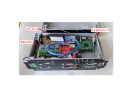
\includegraphics[width=1\textwidth]{./Figures/foto-dispositivo.pdf}
	\caption{Foto del dispositivo de captura en construcción.}
    \label{fig:fotodispositivo}
\end{figure}

\section{Arquitectura de software}
\label{sec:software}

Como se ve en la figura~\ref{fig:bloques}, a la Raspberry Pi entra la señal digital capturada por el analizador lógico en tiempo real, mediante la interfaz USB. Para recibir esta señal se utiliza Sigrok, invocándolo de la siguiente manera:

\begin{lstlisting}
sigrok-cli -d fx2lafw --continuous --config samplerate=12m
           --channels D0 -O binary
\end{lstlisting}

Este comando recibe la señal del VKTECH en la interfaz USB, muestrea la señal digital con una frecuencia de 12 MHz y produce como salida un flujo de datos que se puede redireccionar a un archivo o a un \textit{pipe} de Unix.
Por cada muestra capturada, se emite un byte en el que el bit menos significativo es 0 o 1 dependiendo de si la señal lógica capturada es baja o alta.
De esta forma, el flujo de datos tiene un ancho de banda de 12 MB/s, aunque solo se usa uno de los 8 bits de cada byte.
En la figura~\ref{fig:sigrok} se muestra un ejemplo del flujo de datos producido por Sigrok.

\begin{figure}[htbp]
	\centering
    {
        \fontfamily{phv}
        \fontsize{8pt}{8pt}\selectfont
        \input{./Figures/sigrok.pdf_tex}
    }
	\caption{Flujo de datos producido por Sigrok.}
    \label{fig:sigrok}
\end{figure}

El software que corre en la Raspberry Pi está programado en lenguaje Go y su código fuente está disponible en la plataforma Github \cite{mvbparse-go}.

\section{Dispositivo generador de señal}
\label{sec:generador}
